\documentclass[10pt,a4paper]{article}
\usepackage[utf8]{inputenc}
\usepackage{amsmath}
\usepackage{amsfonts}
\usepackage{amssymb}
\usepackage{fourier}
\usepackage{cleveref}
\usepackage{tikz}
\usepackage{listings}
\usepackage{float}
\author{Daniel Underwood}
\title{Linear System Solution of Poisson Equation on Dirichlet Boundary}

\newcommand{\crefrangeconjunction}{--}

\usepackage{color} %red, green, blue, yellow, cyan, magenta, black, white
\definecolor{mygreen}{RGB}{28,172,0} % color values Red, Green, Blue
\definecolor{mylilas}{RGB}{170,55,241}


\begin{document}
\maketitle

\lstset{language=Matlab,%
    %basicstyle=\color{red},
    breaklines=true,%
    morekeywords={matlab2tikz},
    keywordstyle=\color{blue},%
    morekeywords=[2]{1}, keywordstyle=[2]{\color{black}},
    identifierstyle=\color{black},%
    stringstyle=\color{mylilas},
    commentstyle=\color{mygreen},%
    showstringspaces=false,%without this there will be a symbol in the places where there is a space
    numbers=left,%
    numberstyle={\small \color{gray}},% size of the numbers
    numbersep=9pt, % this defines how far the numbers are from the text
    emph=[1]{for,end,break},emphstyle=[1]\color{red}, %some words to emphasise
    %emph=[2]{word1,word2}, emphstyle=[2]{style},    
}

\section*{Introduction}
The Dirichlet boundary value problem is a boundary value problem in which the function on the boundary is defined by a function; that is

\begin{subequations}
  \begin{align}
  \hat{\mathcal{D}} u(x_1 , ... , x_n) &= f(x_1 , ... , x_n) \label{eqn: dirichlet 1}\\
  u(x_1, ..., x_n) &= g(x_1, ..., x_n) \,\, \text{for} \,\, (x_1, ..., x_n) \in \partial\Omega \label{eqn: dirichlet 2}
  \end{align}
\end{subequations}

where $\hat{\mathcal{D}}$ is a linear differential operator consisting of a sum of derivatives of any order including mixed derivatives and $u$, $f$, and $g$ are functions of $n$ variables from $\mathbb{R}^n$ to $\mathbb{R}$. The problem is solved on a domain $\Omega \subset \mathbb{R}^n$ with a boundary $\partial \Omega$. An additional constraint of the Dirichlet problem is that $u$ is a harmonic function. In simpler terms, a Dirichlet problem is a boundary value problem in which the solution value is given in terms of a function, rather than other conditions such as the value of the solution's derivative on the boundary that is given in a Neumann problem.

The Dirichlet problem is very useful in a variety of fields. Differential equations frequently used with Dirichlet boundary conditions include the  Laplace equation, Poisson equation, heat/diffusion, and wave equation. These equations are seen quite often and the latter three are actually all more general forms of the Laplace equation; the Poisson equation is a non-homogeneous form while the heat/diffusion and wave equations add first and second time derivative terms, respectively.

The Laplace equation

\begin{equation}
\Delta u = 0 \label{eqn: laplace}
\end{equation}

is one of the most basic partial differential equations used with Dirichlet boundary conditions. The solutions to this equations are harmonic functions. The Laplace equation has uses in various fields of physics to describe potentials due to forces such as gravity, the electromagnetic force, and fluid forces. It it also the steady-state heat or diffusion equation as well as the steady-state wave equation by taking $u_t = 0$ in \cref{eqn: diffusion} or $u_{tt} = 0$ in the $\Box$ operator of \cref{eqn: wave}.

The Poisson equation

\begin{equation}
\Delta u = f \label{eqn: poisson}
\end{equation}

Is the non-homogeneous form of \cref{eqn: laplace}. The Poisson equation has uses throughout physics as $f$ can be used to represent forces such as gravity, electromagnetism, and fluid forces. In these cases, $u$ represents a potential, which can be related to a force via Newton's second law or can be used in energy analysis. The $f$ term comes from a source. In the case of an electrostatic field, we have $f = - \frac{\rho (r)}{\epsilon_0}$, where $\rho$ is the radial charge density; the gravitational source term is $f = 4 \pi^2 G \rho(r)$, where $G$ is the universal gravitational constant and $\rho$ is the radial mass density.

The heat or diffusion equation

\begin{equation}
u_t - a \Delta u = 0 \label{eqn: diffusion}
\end{equation}

is a frequently used partial differential equation to represent the transfer of heat on the domain of a piece of material or the diffusion of a fluid through another fluid. $a$ is either the heat transfer coefficient or the diffusion coefficient depending on the usage case. It is frequently constant as a simplification, but can vary with position or time in more complicated cases. In these cases, the divergence term affects the transfer function and the equation will take on a slightly different form.

The wave equation

\begin{equation}
\Box u = 0 \label{eqn: wave}
\end{equation}

where $\Box \equiv \frac{1}{c^2} \frac{\partial^2}{\partial t^2} - \Delta$ is the d'Alembert operator with $c$ being the wave speed. The wave equation has usage throughout physics. In classical mechanics, the wave equation is used to represent oscillations and is the start to the large field of wave mechanics. Electromagnetism and quantum mechanics have their own wave equations, being Maxwell's equations for electromagnetism and the Schr{\"o}dinger equation in quantum mechanics.

\section*{Mathematical Theory}
There are many ways to solve \crefrange{eqn: laplace}{eqn: wave}. Analytically, they may be solved by separation of variables for many cases and in the case of Dirichlet boundary conditions may be solved by using Green's function; however, both of these techniques can become very difficult or even impossible depending on the domain on which the problem is being solved. Due to this difficulty, numerical methods start becoming highly favorable. While numerical methods do not yield a solution in terms of analytic functions, they can give a good idea of the behavior of the solution and parameters can be adjusted to make the error within an acceptable range. Additionally, once written, numerical methods can be used on a variety of variations of the problem and are often solved much quicker than a human could solve the same equation if a solution exists. Numerical data can even be fitted by functions to make guesses of analytic solutions or approximations.

Numerical solutions represent discrete relations rather than continuous ones and can be formulated by transforming the differential equation into a linear system. In this case, we have Poisson's equation with a Dirichlet boundary on a domain $\Omega \subset \mathbb{R}^2$

\begin{subequations}
  \begin{align}
  -u_{xx} - u_{yy} &= f(x, y) & \\
  u(x, y) &= 0 \,\, \text{for} \,\, (x, y) \in \partial \Omega
  \end{align}
\end{subequations}

The domain $\Omega$ is shown in \cref{fig: domain}. The domain could be scaled to arbitrary sizes, so it is easiest to take the squares making up $\Omega$ to be unit squares.

\begin{figure}[float]
\center
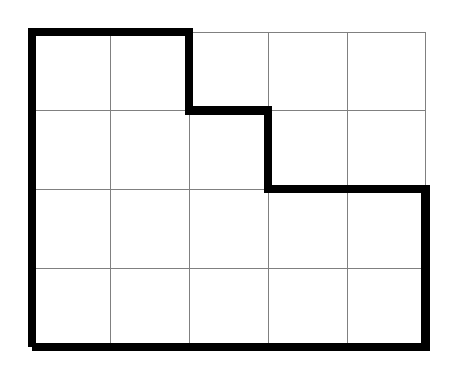
\begin{tikzpicture}
\draw[help lines] (0,0) grid (5,4);
\draw[line width=3] (0,0) -- (5,0) -- (5,2) -- (3,2) -- (3,3) -- (2,3) -- (2,4) -- (0,4) -- (0,0);
\end{tikzpicture}
\caption{Domain $\Omega$}
\label{fig: domain}
\end{figure}

To solve a differential equation numerically, we must discretize the differential operator into steps. A starting point for this is the limit definition of a derivative

\begin{equation}
\label{eqn: limit derivative}
f'(a) = \lim\limits_{h \to 0} \frac{f(a + h) - f(a)}{h}
\end{equation}

To discretize this limit, we take $h \to \Delta h$, where $\Delta h$ is small and taken to be smaller to achieve more accurate results. This relation can be used with a Taylor series to find relations for higher-order derivatives. Applying this to find the Laplace operator for $\mathbb{R}^2$ and indexing values yields the algebraic relation

\begin{equation}
\label{eqn: laplacian algebra}
- \Delta u(x_i, y_j) = \frac{4u_{ij} - u_{i+1, j} - u_{i+1, j} - u_{i, j+1} - u_{i, j-1}}{\left( \Delta h \right)^2}
\end{equation}

With \cref{eqn: laplacian algebra}, an operator matrix $\hat{A}$ may be formed such that $\hat{A} \vec{u}$ is a discretized form of $\Delta u$ for $\vec{u}$ is a vector formed by $u(x_i, y_j)$, where $x_i$ and $y_j$ are  points that are created when the boundary $\Omega$ is separated into a mesh with step size $\Delta h$. We then obtain a linear system

\begin{equation}
\label{eqn: linear system}
\hat{A} \vec{u} = \vec{f}
\end{equation}

where $\vec{f}$ is the vector created from $f(x_i, y_j)$ evaluated at the same mesh points as $\vec{u}$. 

This system can be solved by several different methods. To simplify the computation, the $\Delta h$ term is factored out of $\hat{A}$ and placed with the function term

\begin{equation}
\label{eqn: linear system 2}
\tilde{\hat{A}} \vec{u}  = \left( \Delta h \right)^2 \vec{f}
\end{equation}

 where $\tilde{\hat{A}} \equiv \left( \Delta h \right)^{-2} \hat{A}$. With this system defined by the operator in \cref{eqn: laplacian algebra}, we have an error of order $\left( \Delta h \right)^4$.

\section*{Computational Details}
To solve this problem numerically, MATLAB code was used. Relevant code is shown and the entire function used is attached.

The first step to solving this problem numerically is to create the domain and split it into a mesh based on a step size, which is $\Delta h$ in \cref{eqn: laplacian algebra}. In the code, this was done by using a matrix to represent the unit squares of the domain. For example, the matrix that represents the domain of interest shown in \cref{fig: domain} is given by

\begin{displaymath}
\left[
\begin{matrix}
1 & 1 & 0 & 0 & 0 \\
1 & 1 & 1 & 0 & 0 \\
1 & 1 & 1 & 1 & 1 \\
1 & 1 & 1 & 1 & 1
\end{matrix}
\right]
\end{displaymath}

As can be seen, the matrix is in $\mathbb{R}^{m \times n}$ where $m$ is the maximum $y$ value of the domain and $n$ is the maximum $x$ value of the domain if the domain is split into unit squares. Within the matrix, a $1$ represents a unit square while a $0$ represents a place that is not in the domain. Using this method, it is easy to use an arbitrary domain. The matrix can be of any dimension and the size can be scaled to more accurately represent features such as curves. This way of representing the domain can even deal with domains with features such as holes.

When the domain is split up into smaller pieces, the unit squares of the domain simply repeat $\frac{1}{\Delta h}$ times in both their column and the next row. For example, when a step size of $\Delta h = \frac{1}{2}$ is used, the above matrix undergoes the transformation

\begin{displaymath}
\left[
\begin{matrix}
1 & 1 & 0 & 0 & 0 \\
1 & 1 & 1 & 0 & 0 \\
1 & 1 & 1 & 1 & 1 \\
1 & 1 & 1 & 1 & 1
\end{matrix}
\right]
\to
\left[
\begin{matrix}
1 & 1 & 1 & 1 & 0 & 0 & 0 & 0 & 0 & 0 \\
1 & 1 & 1 & 1 & 0 & 0 & 0 & 0 & 0 & 0 \\
1 & 1 & 1 & 1 & 1 & 1 & 0 & 0 & 0 & 0 \\
1 & 1 & 1 & 1 & 1 & 1 & 0 & 0 & 0 & 0 \\
1 & 1 & 1 & 1 & 1 & 1 & 1 & 1 & 1 & 1 \\
1 & 1 & 1 & 1 & 1 & 1 & 1 & 1 & 1 & 1 \\
1 & 1 & 1 & 1 & 1 & 1 & 1 & 1 & 1 & 1 \\
1 & 1 & 1 & 1 & 1 & 1 & 1 & 1 & 1 & 1
\end{matrix}
\right]
\end{displaymath}

For this reason, we must choose $\Delta h \leq 1$, although it is already known that a smaller $\Delta h$ yields better results. This expansion of matrices is handled by several nested loops and conditional statements in the MATLAB code

\lstinputlisting[language=Matlab, firstline=17, lastline=37, firstnumber=17]{centralDifferencePoisson.m}

While loops and conditional statements are a cornerstone of many numerical methods, there is a likelihood that this code could be modified to perform fewer iterations for greater performance.

The next step in the process of solving the equations is to form a list of mesh points in the domain since what we have only represents unit squares within the domain. The mesh points of the domain are given by the intersection of four squares. Therefore, the mesh points could be found by searching for every $2 \times 2$ matrix in the domain matrix such that all the elements are $1$. However, it may also be calculated for this domain by checking the element to the upper right corner of the current element and making sure each is $1$. This is done in the code by a simple conditional at each element of the matrix

\lstinputlisting[language=Matlab, firstline=58, lastline=71, firstnumber=58]{centralDifferencePoisson.m}

The coordinates of the mesh point are given by the location of the element of the unit square to the top right of the mesh point scaled by $\Delta h$. Shifting of the index is done in the code as the matrices are indexed starting at $(1,1)$ and our domain starts at $(0,0)$. The row of the mesh point in the matrix created by this code corresponds to the row of the solution value in $\vec{u}$ for that mesh point.

The next step is to create the operator matrix $\tilde{\hat{A}}$. Due to the $4u_{ij}$ term in \cref{eqn: laplacian algebra}, it is known that the diagonals of $\tilde{\hat{A}}$ are 4, so an identity matrix is created and multiplied by $4$. For the rest of the elements of the matrix, the matrix-vector multiplication must be checked for mesh points adjacent to the current element. This is done in the code with a long conditional statement at each mesh point

\pagebreak
\lstinputlisting[language=Matlab, firstline=78, lastline=92, firstnumber=78]{centralDifferencePoisson.m}

This is another area of the code that requires many calls and evaluations of conditional statements. It is expected that significant performance improvements could be made here.

The final step before solving the linear system with MATLAB's built-in functions is to form the right-hand side of \cref{eqn: linear system 2}. This is simply done by evaluating $f(x,y)$ at each of the mesh points and put the results in an array and multiply that array by $\left( \Delta h \right)^2$. This is done in the code by a very simple loop

\lstinputlisting[language=Matlab, firstline=96, lastline=99, firstnumber=96]{centralDifferencePoisson.m}

Now, the linear system is ready to be solved using built-in functions.

\section*{Conclusion}

The code presented in this report was used to solve the Poisson equation with the right hand sides

\begin{subequations}
\begin{align}
f(x, y) =& x e^{-x^2 - y^2} \label{eqn: gaussian}\\
f(x, y) =& x \left( x - y \right)^3 \label{eqn: cubic}
\end{align}
\end{subequations}

with $\Delta h = \frac{1}{32}$. The solution plots were then compared with the solutions found by MATLAB's PDE toolbox. These plots are shown in \crefrange{fig: gaussian solutions}{fig: pdetool cubic solutions} on the next two pages.


\pagebreak
\subsection*{Solution Plots}

\begin{figure}[H]
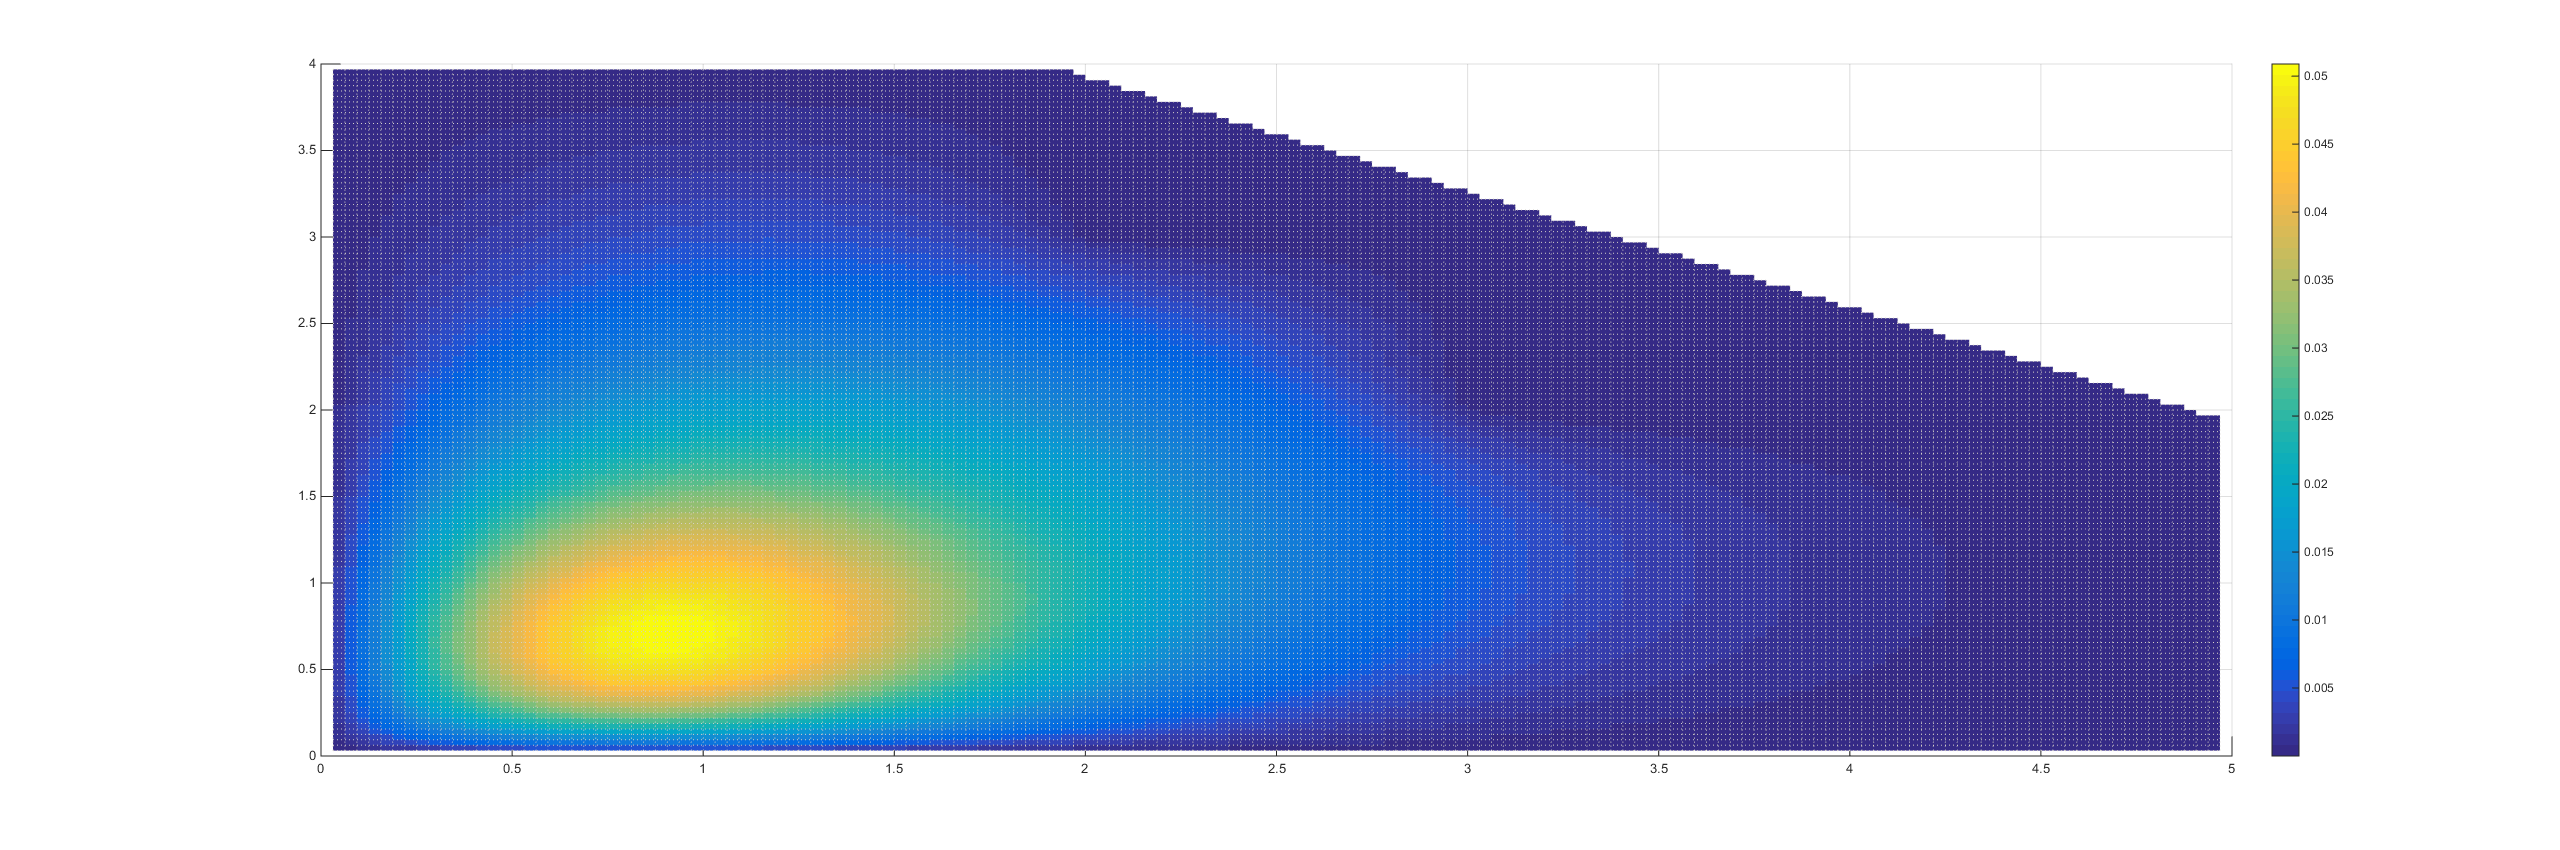
\includegraphics[width=\linewidth]{gaussian-top.png}
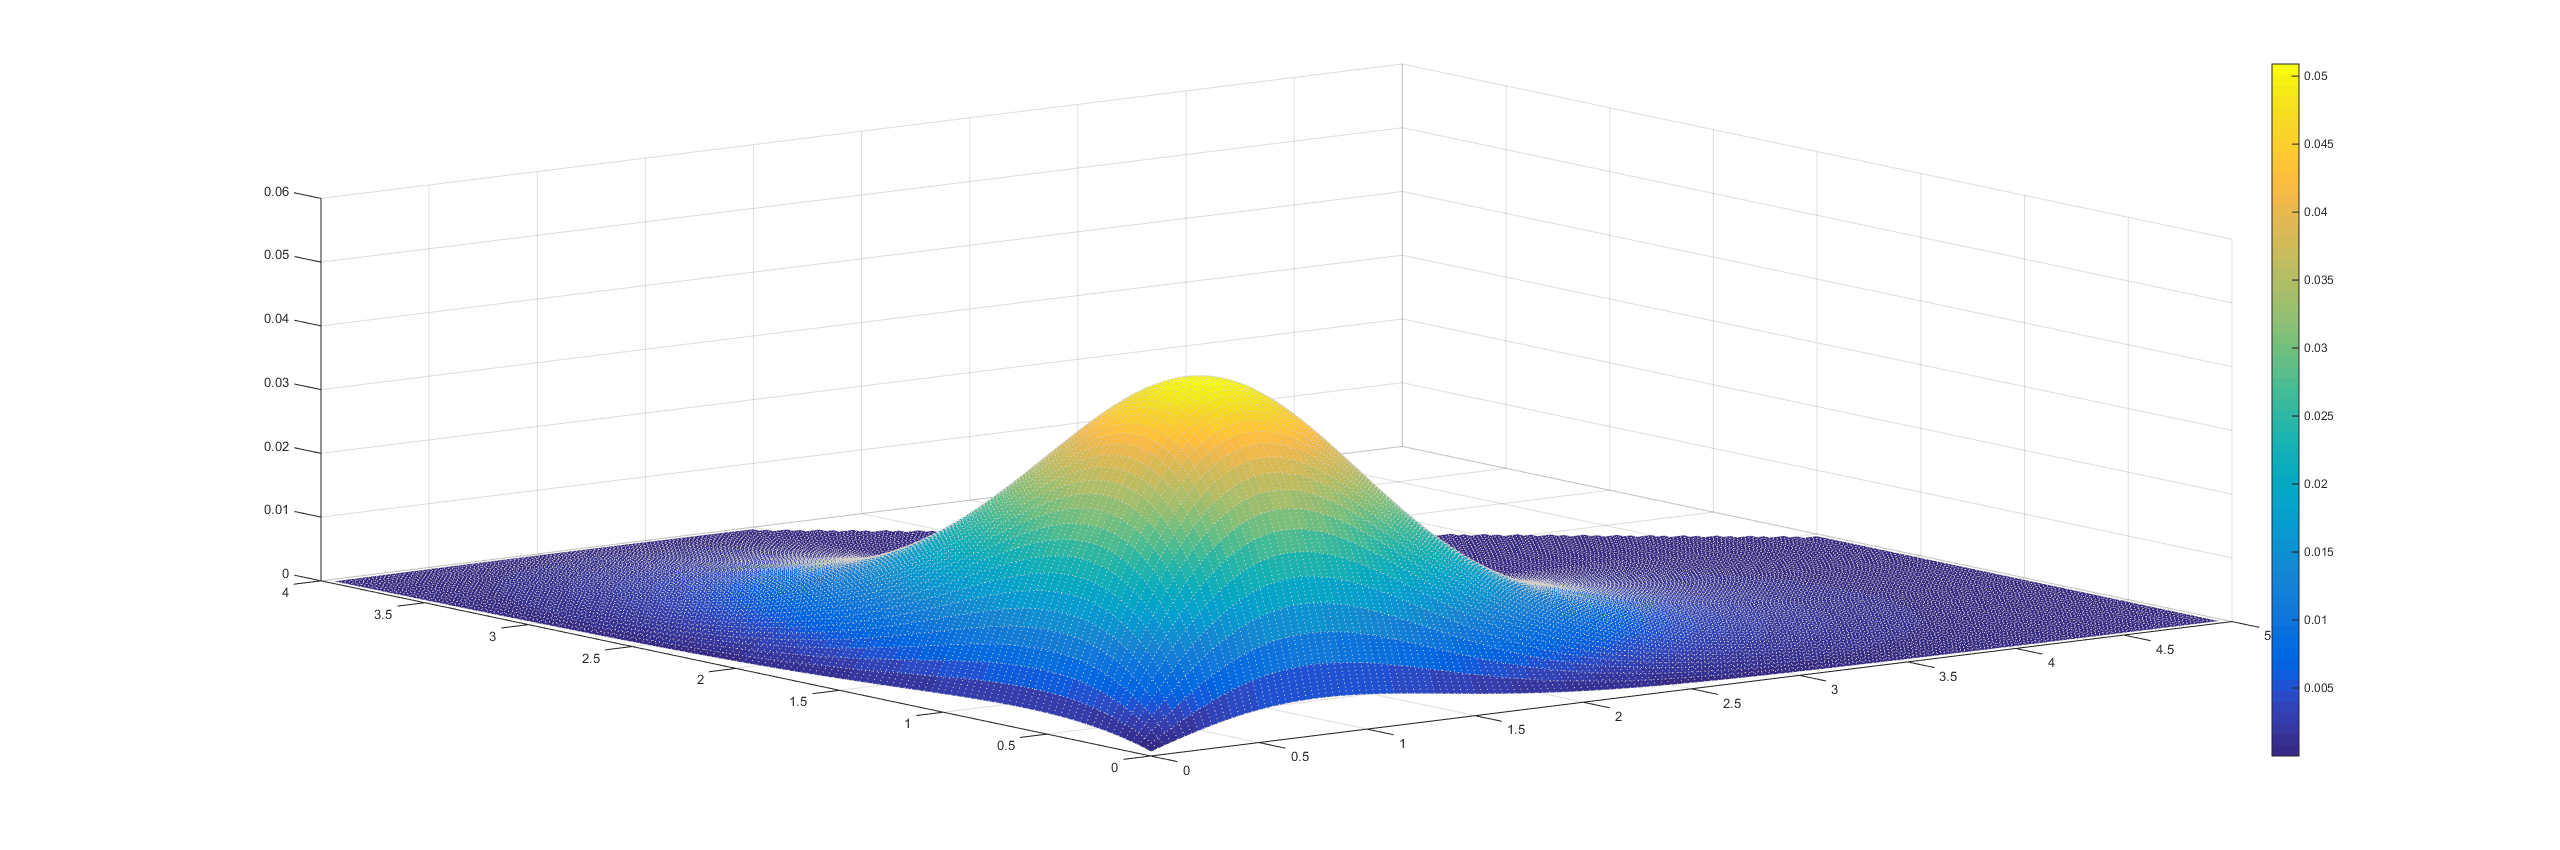
\includegraphics[width=\linewidth]{gaussian-iso.png}
\caption{Solutions to \Cref{eqn: gaussian}}
\label{fig: gaussian solutions}
\end{figure}

\begin{figure}[H]
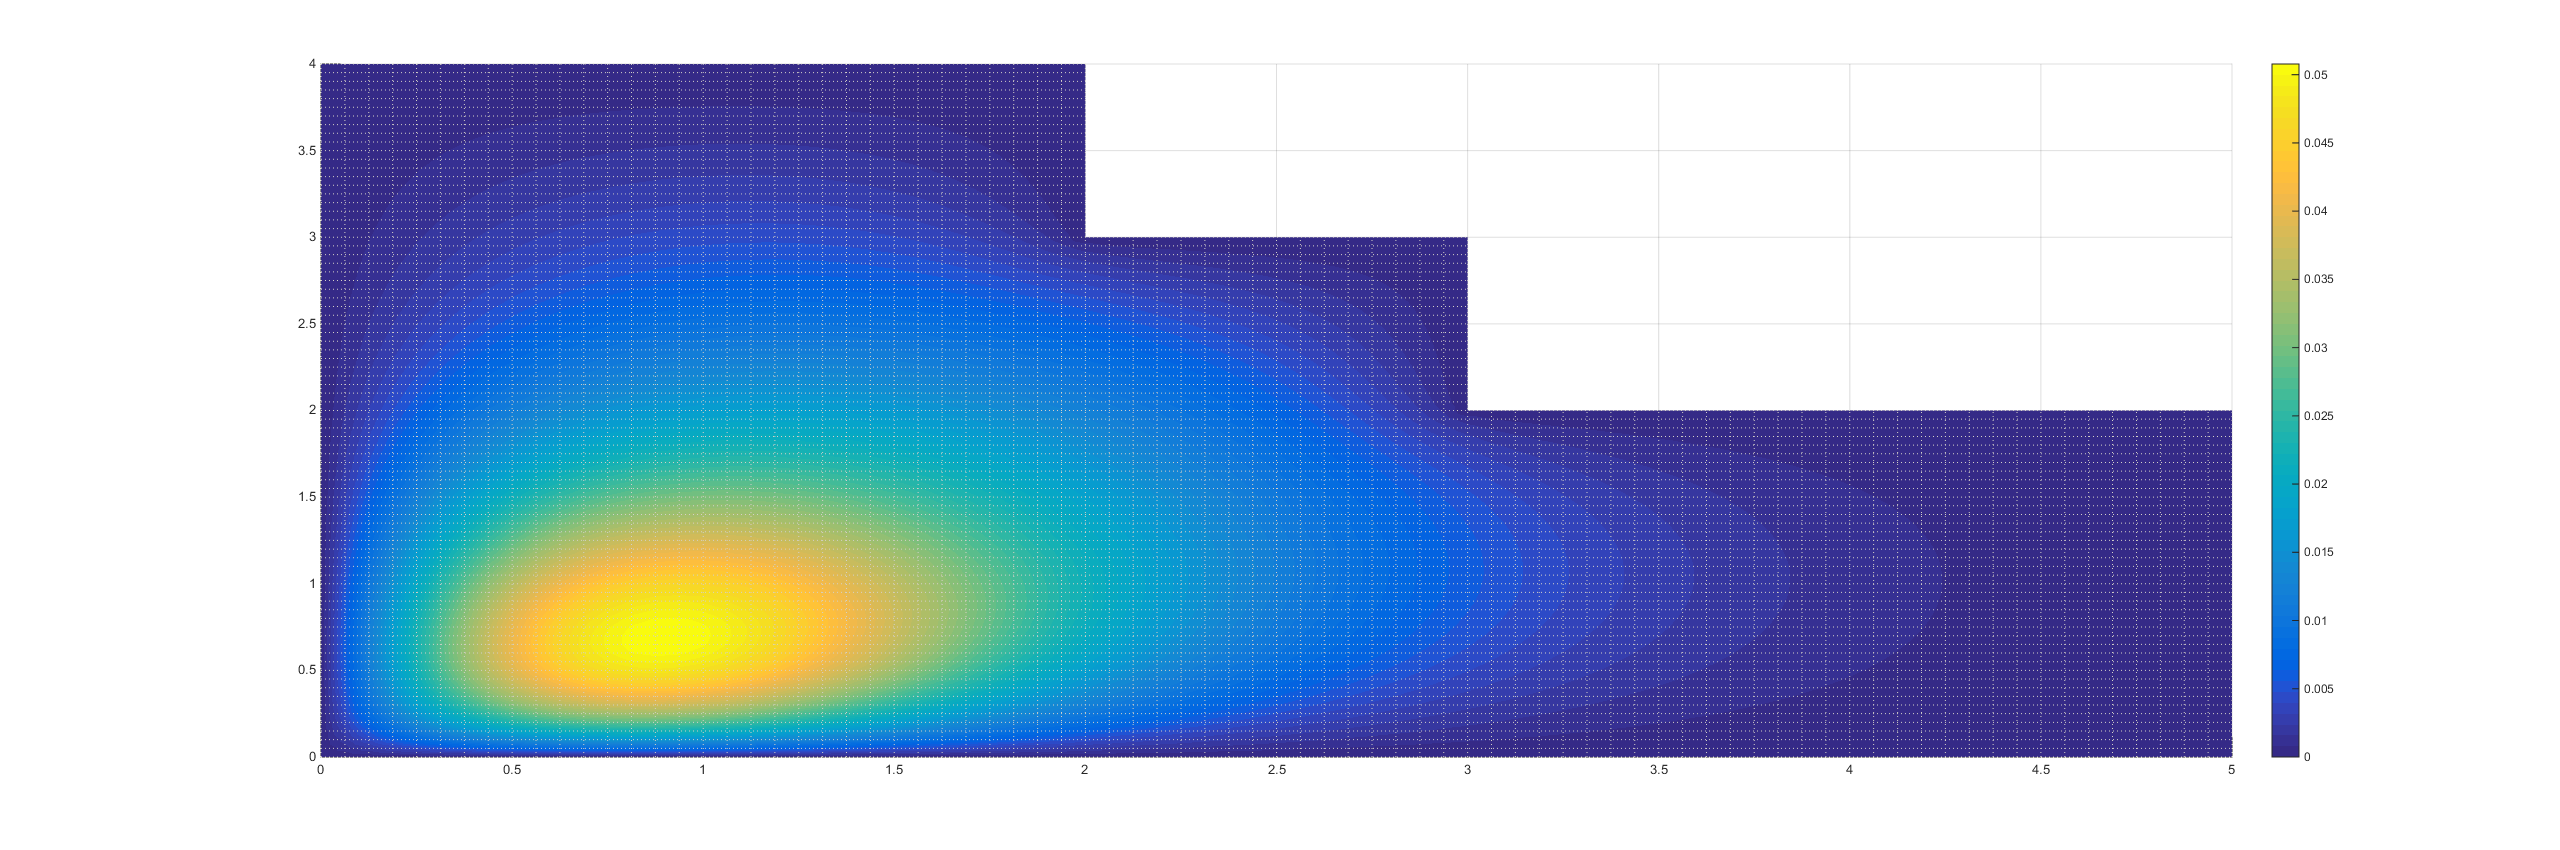
\includegraphics[width=\linewidth]{gaussian-top-pdetool.png}
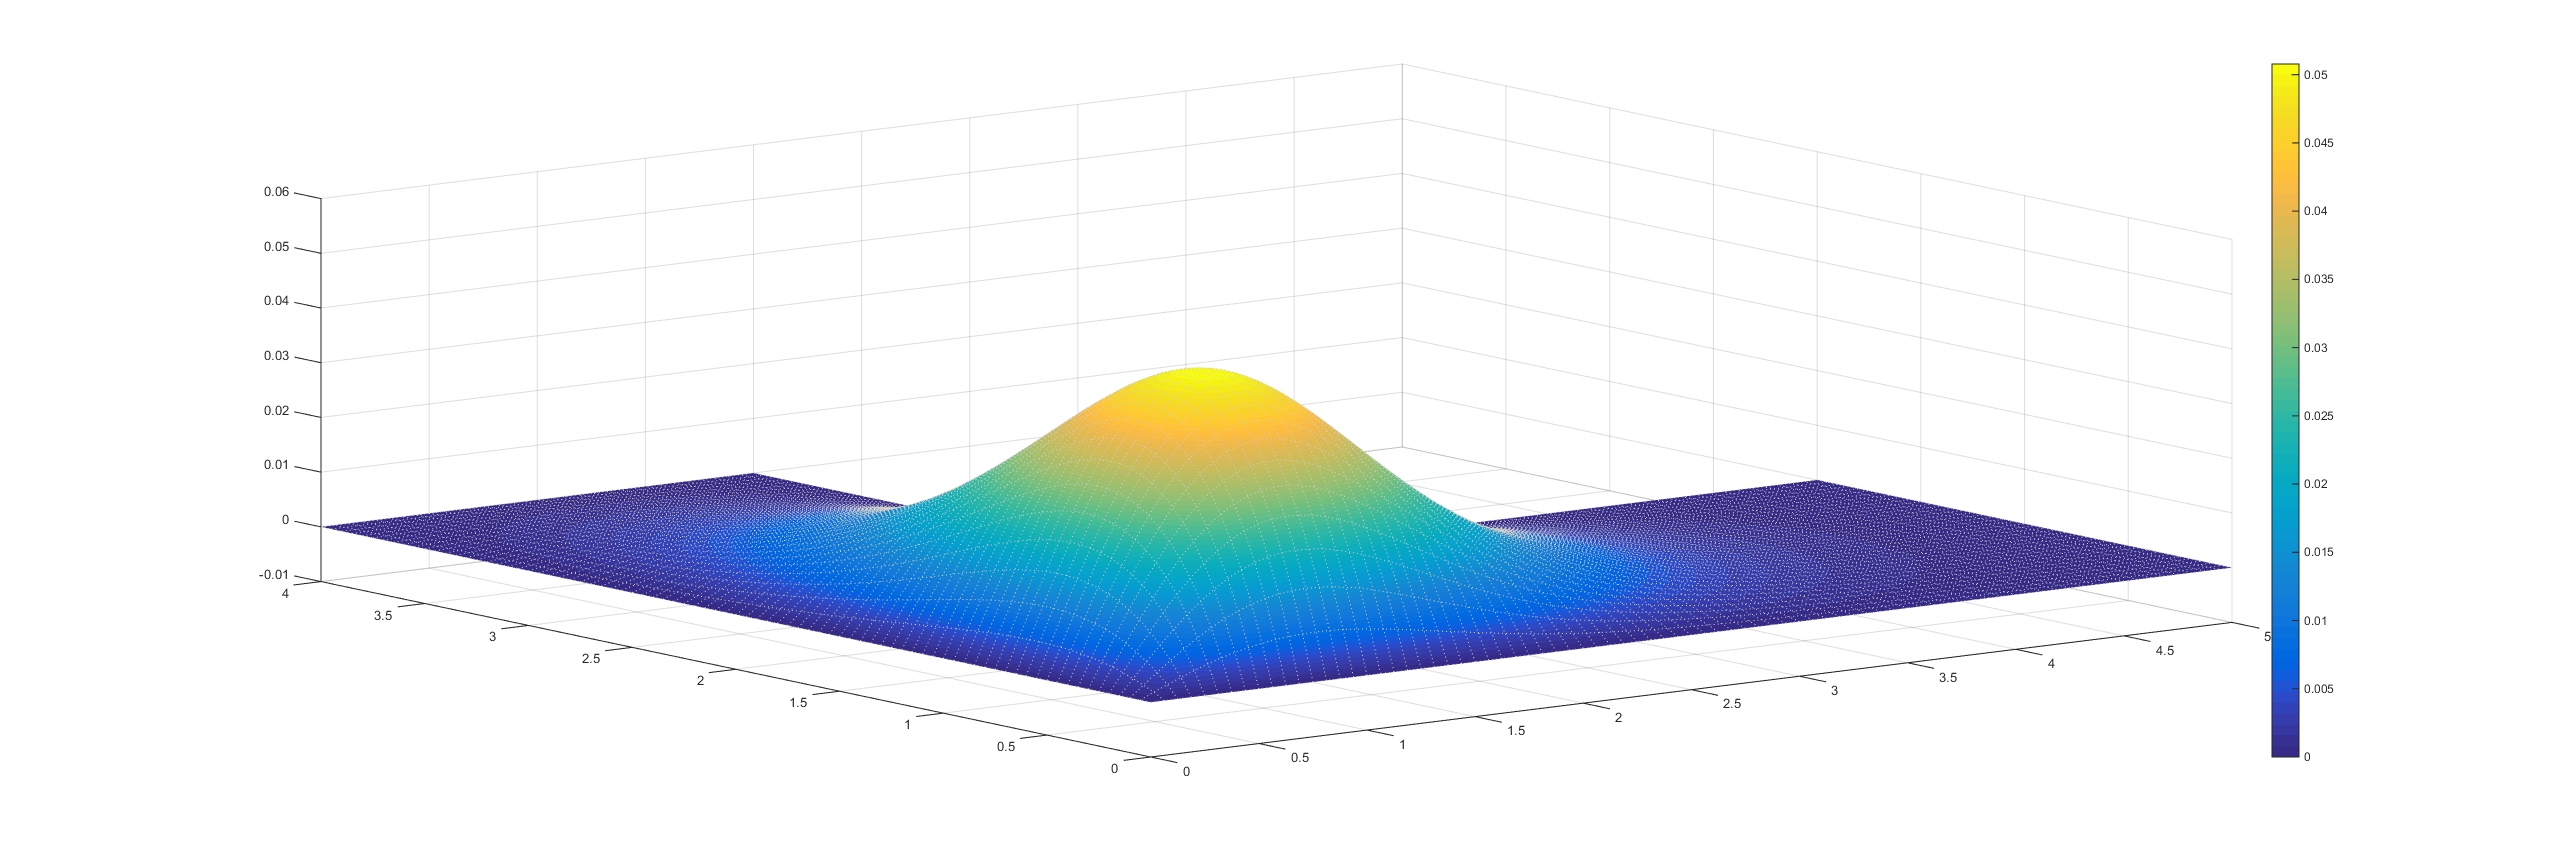
\includegraphics[width=\linewidth]{gaussian-iso-pdetool.png}
\caption{PDE Toolbox Solutions to \Cref{eqn: gaussian}}
\label{fig: pdetool gaussian solutions}
\end{figure}

\begin{figure}[H]
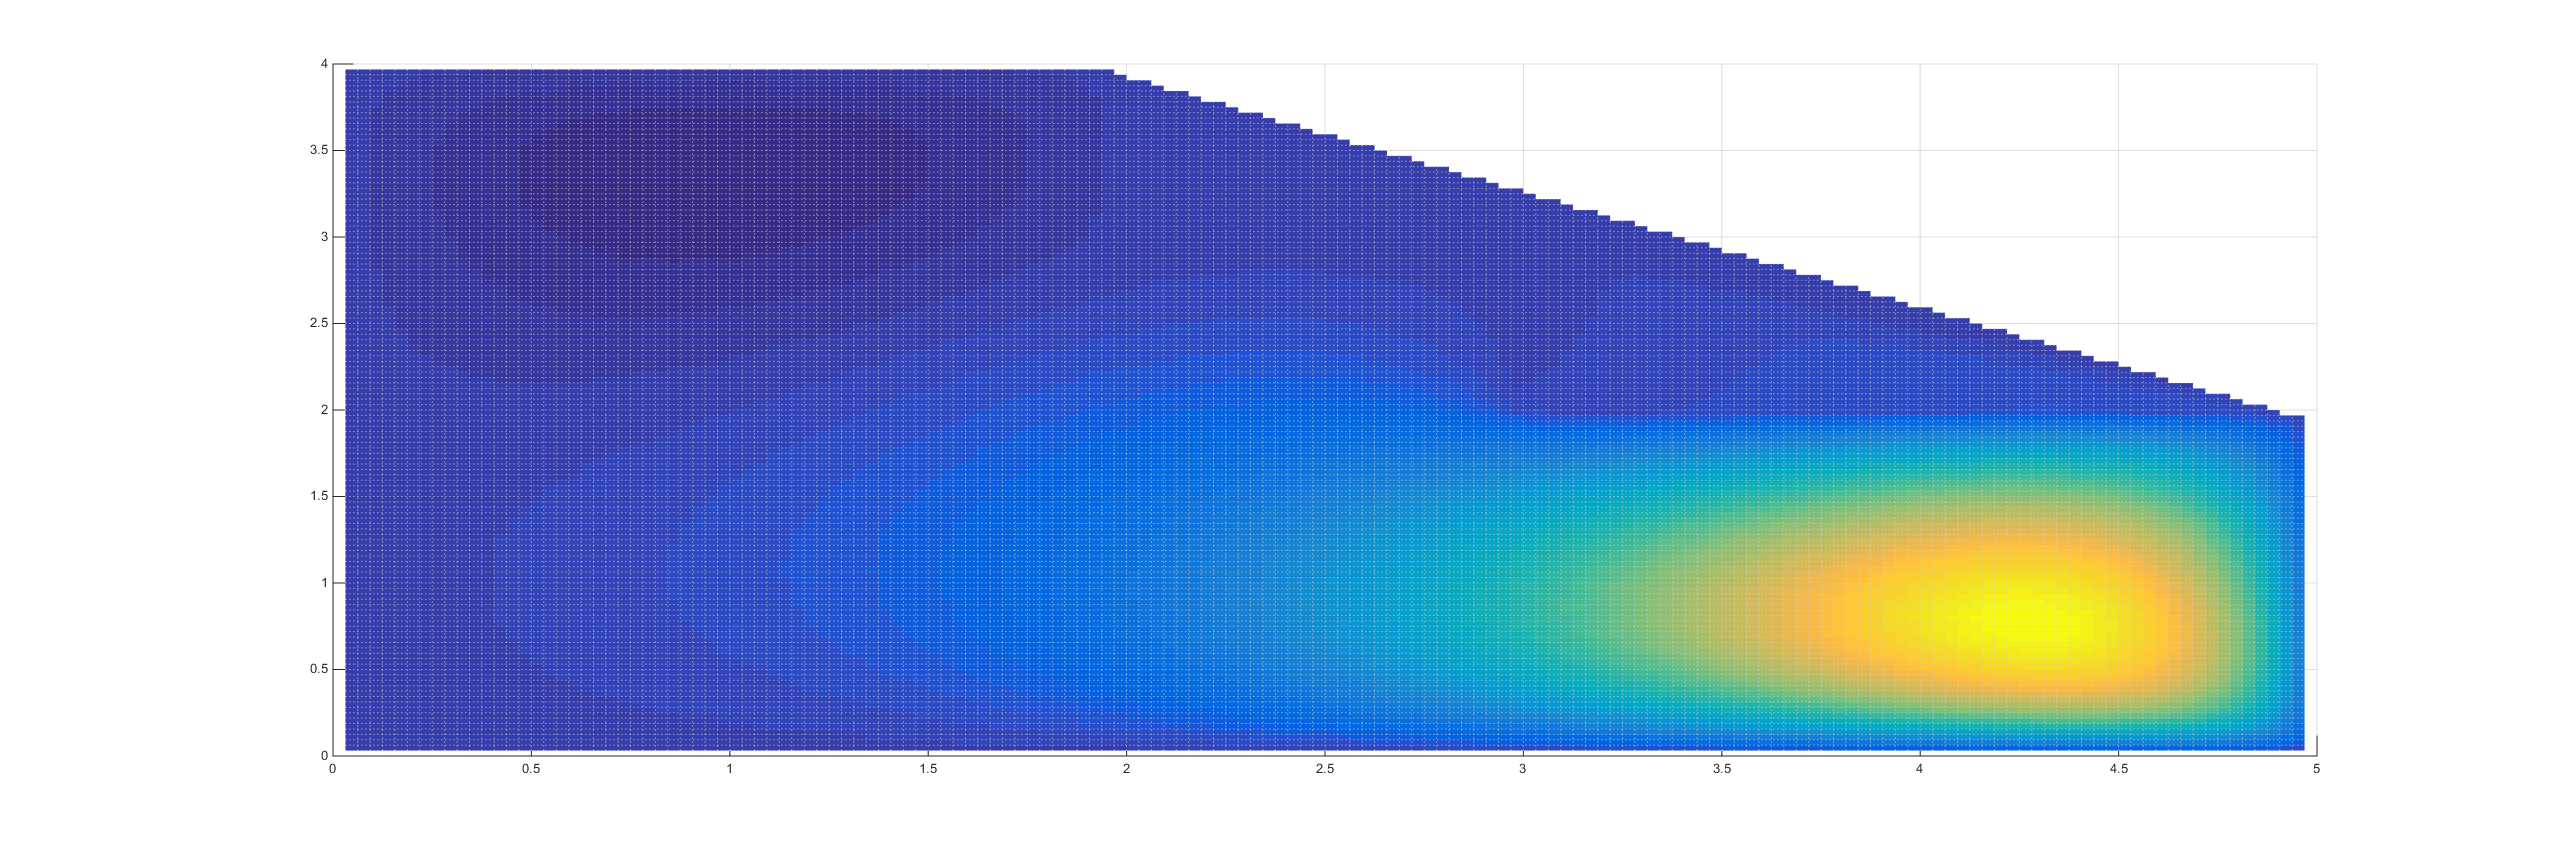
\includegraphics[width=\linewidth]{cubic-top.png}
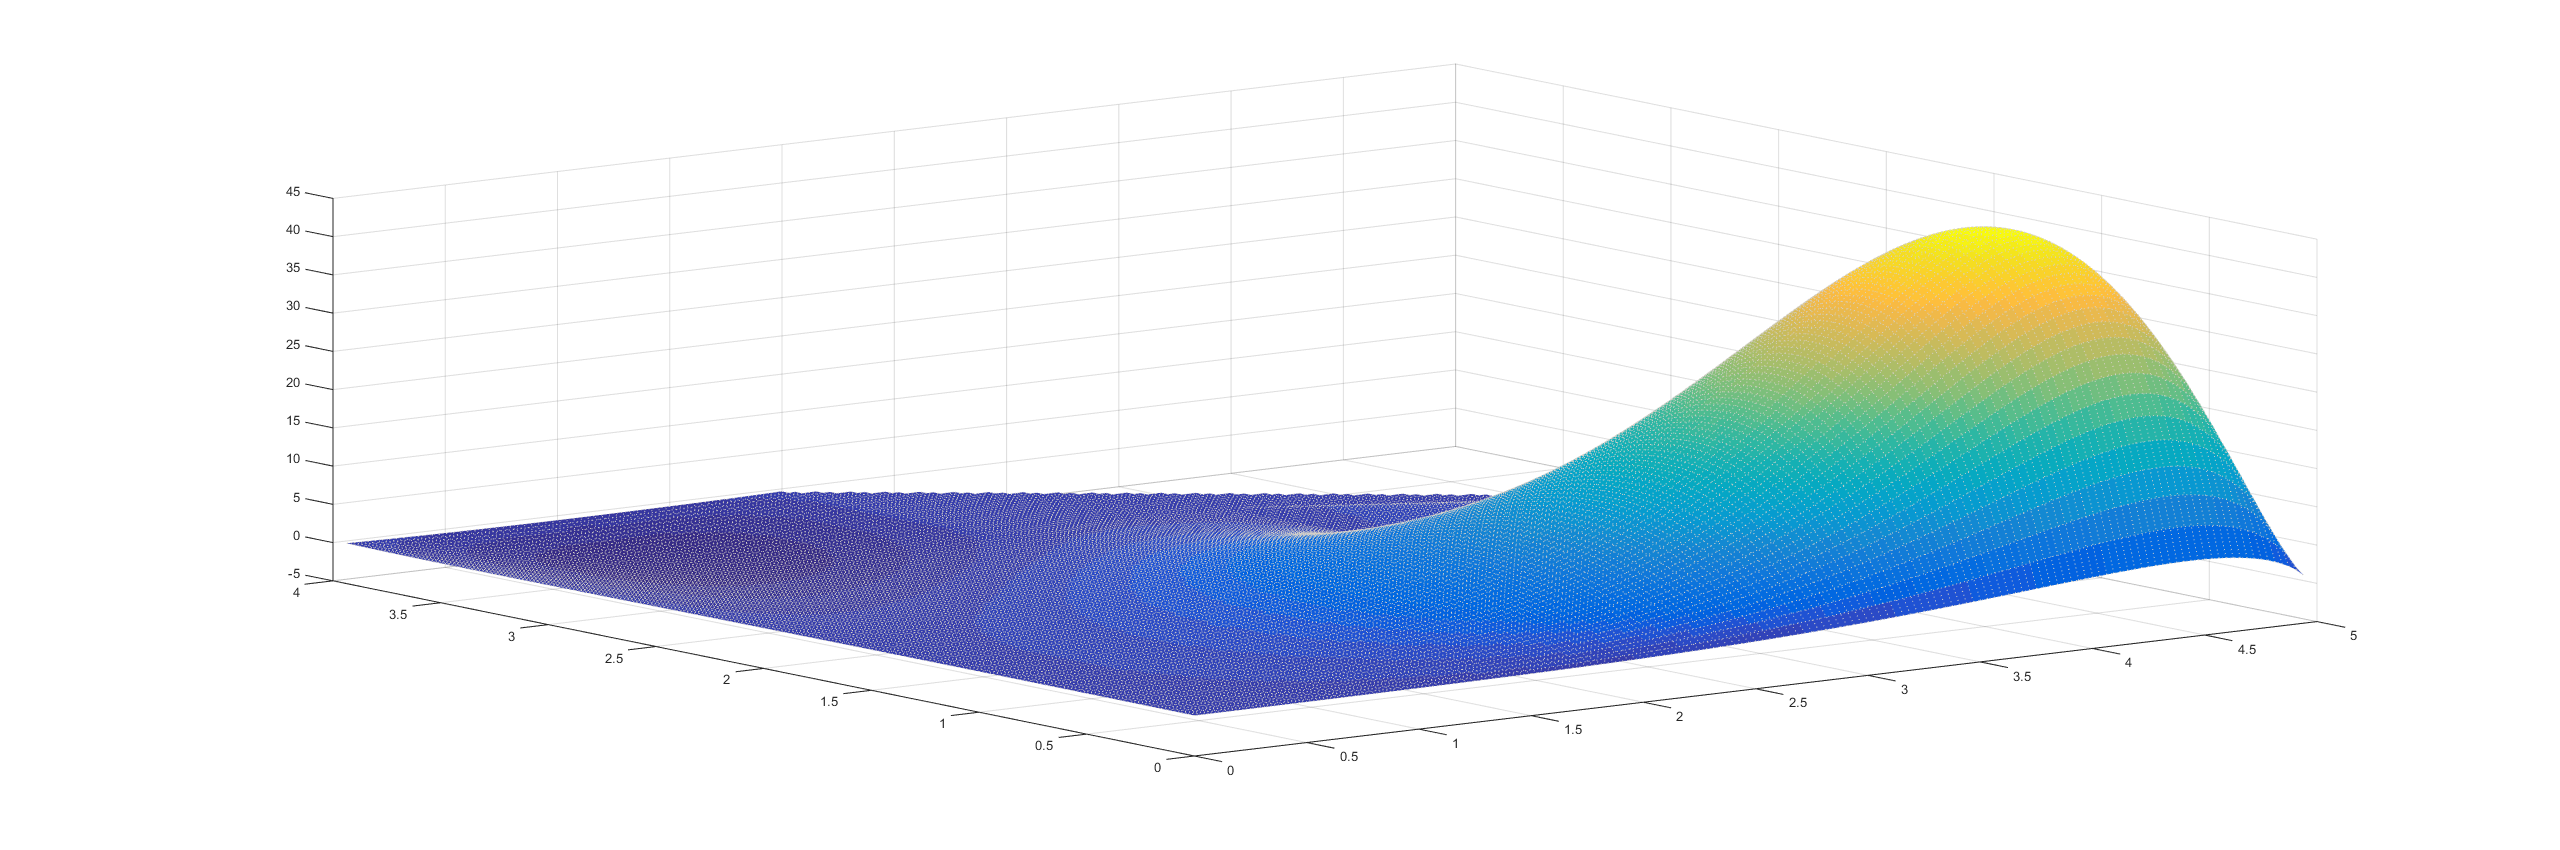
\includegraphics[width=\linewidth]{cubic-iso.png}
\caption{Solutions to \Cref{eqn: cubic}}
\label{fig: cubic solutions}
\end{figure}

\begin{figure}[H]
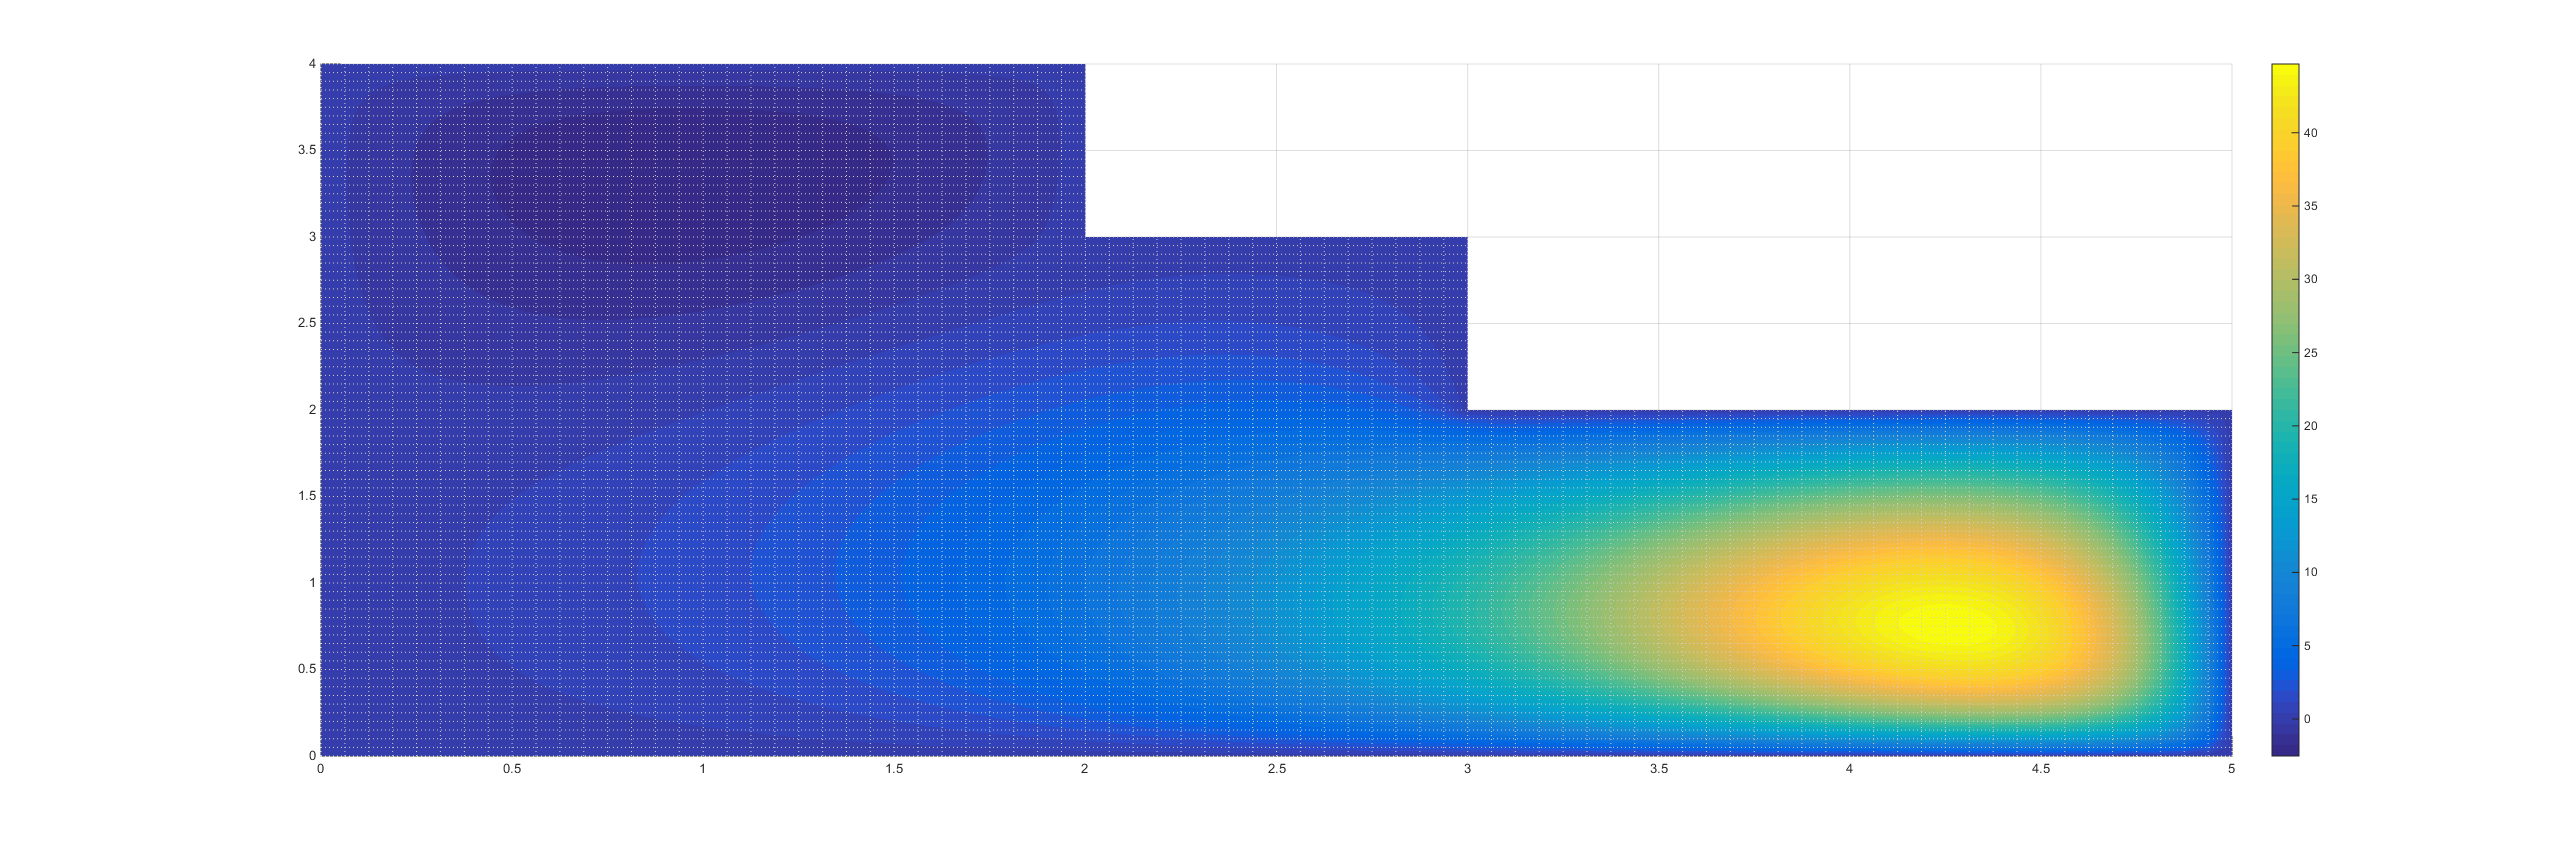
\includegraphics[width=\linewidth]{cubic-top-pdetool.png}
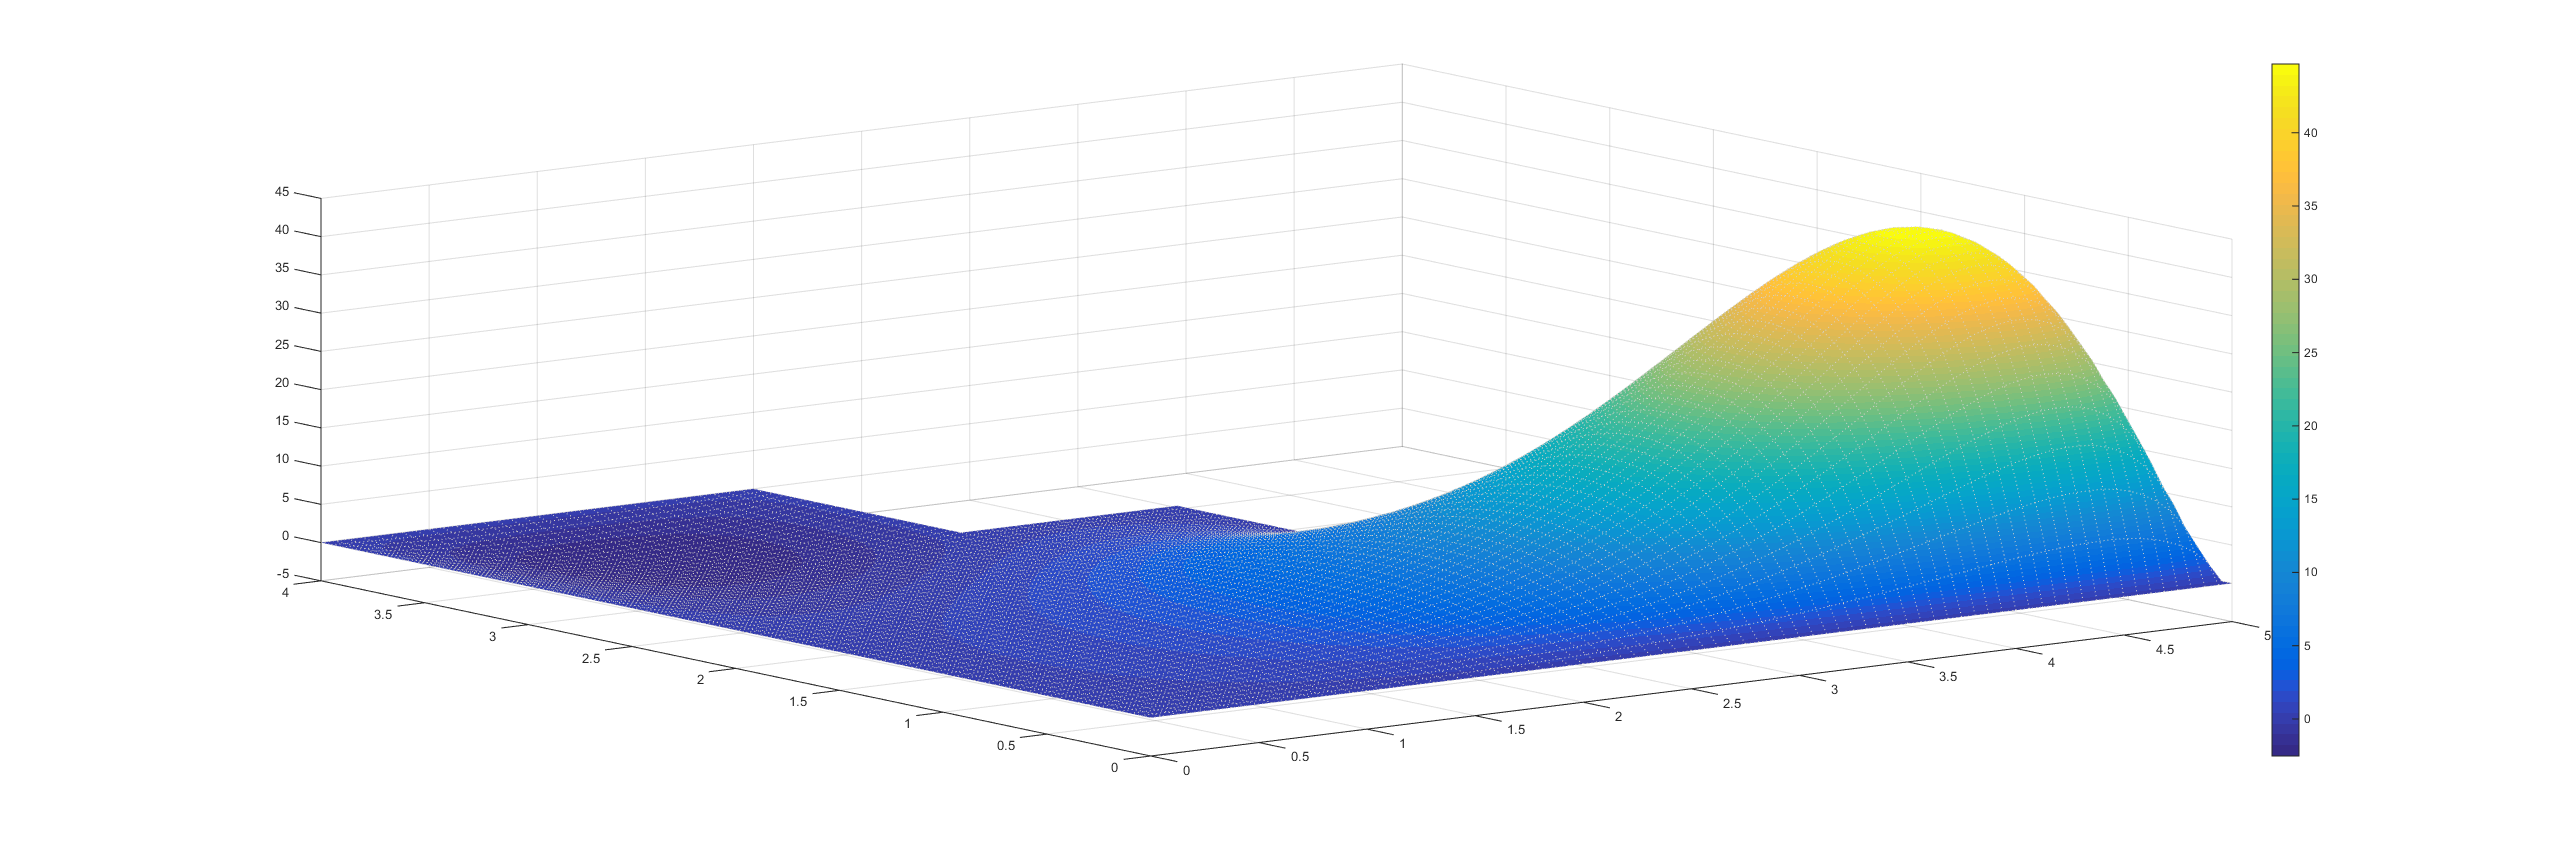
\includegraphics[width=\linewidth]{cubic-iso-pdetool.png}
\caption{PDE Toolbox Solutions to \Cref{eqn: cubic}}
\label{fig: pdetool cubic solutions}
\end{figure}

In both of these cases, it is seen that both MATLAB's PDE toolbox and the code presented in this report found similar solutions with two visible differences -- domain and boundary values.

The difference in the domains is that the PDE toolbox plots the boundary used as an input while the code presented here interpolates the steps at the edge of the boundary. This is due to the way MATLAB requires a matrix to plot a surface and the conversion of coordinate vectors to matrices as done in the code

\lstinputlisting[language=Matlab, firstline=105, lastline=107, firstnumber=105]{centralDifferencePoisson.m}

It can be seen  at the wrapping near the first step that the equation was solved on the correct domain and the only difference is the extra plotted area.

The second issue is the boundary conditions around $(0, 0)$. In the toolbox solutions, they are fixed as they should be, but  differ slightly in the solutions generated by the presented code; this discrepancy decreases as the step size is taken to be smaller.

Overall, this method generates very good results with the differential equation and boundary in this case. Due to the flexible nature of how the domain was implemented, it is expected that this method would work for many other domains. Compared to MATLAB's PDE toolbox, the results are slightly worse although the code is likely much simpler. This method also requires more time to run than the solver used in the toolbox. This could likely be improved by carefully profiling the code and adding threading support.

\newpage
\section*{Full Code Listing}
\lstinputlisting[language=Matlab]{centralDifferencePoisson.m}
\end{document}